% !TEX program = lualatex
\documentclass[12pt,a4paper]{article}

% --------------------- Preamble ---------------------
\usepackage{fontspec}
\setmainfont{TeX Gyre Termes}
\usepackage{microtype}
\usepackage{geometry}
\geometry{margin=1.1in}
\usepackage{setspace}
\usepackage{parskip}
\usepackage{titlesec}
\usepackage{tocloft}
\usepackage{amsmath,amssymb,amsfonts,amsthm,mathtools,bm}
\usepackage{hyperref}
\hypersetup{colorlinks=true, linkcolor=blue, urlcolor=blue, citecolor=blue}
\usepackage{graphicx}
\usepackage{upgreek}
\usepackage{verbatim}
\usepackage{booktabs}
\usepackage{caption}
\usepackage{subcaption}
\usepackage{tikz}
\usetikzlibrary{arrows.meta, positioning, calc, shapes.geometric, decorations.pathmorphing}
\usepackage{enumitem}
\usepackage{float}
\usepackage{csquotes}

% Numbering and section styling
\titleformat{\section}{\large\bfseries}{\thesection.}{0.6em}{}
\titleformat{\subsection}{\normalsize\bfseries}{\thesubsection.}{0.6em}{}
\titleformat{\subsubsection}{\normalsize\itshape}{\thesubsubsection.}{0.6em}{}
\setlist{leftmargin=1.2em}

% Theorem environments
\numberwithin{equation}{section}
\theoremstyle{definition}
\newtheorem{definition}{Definition}[section]
\newtheorem{assumption}{Assumption}[section]
\newtheorem{example}{Example}[section]
\theoremstyle{plain}
\newtheorem{proposition}{Proposition}[section]
\newtheorem{theorem}{Theorem}[section]
\newtheorem{lemma}{Lemma}[section]
\newtheorem{corollary}{Corollary}[section]
\theoremstyle{remark}
\newtheorem{remark}{Remark}[section]

% Shortcuts
\newcommand{\M}{\mathbb{M}}
\newcommand{\inner}[2]{\left\langle #1, #2 \right\rangle}
\newcommand{\norm}[1]{\left\lVert #1 \right\rVert}
\newcommand{\diverg}{\nabla\!\cdot}
\newcommand{\grad}{\nabla}
\newcommand{\curl}{\nabla\times}
\newcommand{\E}{\mathsf{E}}
\newcommand{\D}{\mathsf{D}}

% Title
\title{\Huge\textbf{Wordless Imageless Thought}\\[0.35em]
\Large A Field-Theoretic Interpretation of Aphantasia, Anendophasia, and Embodied Stigmergy within the Relativistic Scalar--Vector Plenum}
\author{Flyxion}
\date{\today}

% --------------------- Document ---------------------
\begin{document}
\maketitle
\begin{spacing}{1.15}

\begin{abstract}
\noindent
This monograph develops a rigorous field-theoretic model of cognition in the absence of phenomenological imagery or inner speech, integrating aphantasia, anendophasia, Arnie Cox’s Mimetic Hypothesis and Mimetic Motor Imagery (MMI), oscillatory neurodynamics, and environmental stigmergy within the Relativistic Scalar--Vector Plenum (RSVP). We formalize cognition on a compact Riemannian manifold $\M$ with metric $g_{\mu\nu}$, where scalar potential $\Phi$ (semantic intensity), vector flow $\bm{\mathcal v}$ (directed cognitive currents), and entropy density $S$ (configurational complexity) evolve by coupled PDEs. Visual/auditory imagination are treated as \emph{mimetic projection layers}---$\pi_V,\pi_A$---whose suppression (aphantasia/anendophasia) preserves semantic computation via direct entropic descent. We introduce amplitwistor modes for midbrain-gated synchronization, TARTAN (Trajectory-Aware Recursive Tiling with Annotated Noise) for multiscale entropy geometry, and CLIO (Cognitive Loop via In-Situ Optimization) for adaptive gain control. We prove an H-theorem analog, give local well-posedness, present falsifiable predictions (e.g., diagramming interventions equalize spatial task performance with $d < 0.1$; CLIO gain $\kappa_{\mathrm{CLIO}}$ negatively correlates with VVIQ score, $r < -0.5$), and derive coupled internal--external field equations for stigmergic memory. We conclude with implications for neurodiversity, AI design, and philosophy of mind. Figures (TikZ) schematize manifold decompositions, loops, and bifurcations.
\end{abstract}

\tableofcontents
\newpage

% --------------------- 1. INTRODUCTION ---------------------
\section{Introduction}\label{sec:intro}
Cognitive science has often assumed that conscious thinking requires phenomenological substrates---mental images, inner speech, or stepwise propositional rehearsal. Reports of aphantasia (absent voluntary imagery) and anendophasia (absent inner speech) challenge that assumption while preserving competence in reasoning, planning, and creativity. We argue these conditions reveal a more primitive mode of cognition: \emph{direct traversal of semantic geometry without mimetic rendering}. Within RSVP, imagery and inner speech are not constitutive of thought; they are optional projections that some agents forgo without functional loss.

Historically, this view resonates with strands from Kantian faculties, Wittgensteinian practice-based meaning, and contemporary 4E cognition, while being grounded in neurophysiology: large-scale oscillations, cortico-subcortical loops, and embodied action. We integrate Cox’s Mimetic Hypothesis and MMI: imagination leverages covert motor simulation; perception and understanding are enacted through the body. In RSVP, these embodied flows are formalized as vector field dynamics coupled to $\Phi$ and $S$, with external artifacts acting as writable memory: \emph{stigmergy}.

\vspace{0.3em}
\noindent\textbf{Contributions.} We:
\begin{enumerate}[label=(\alph*)]
\item Formalize RSVP fields on $\M$ and prove local existence/uniqueness for the core PDEs.
\item Introduce mimetic projection operators and show their suppression preserves semantic computation.
\item Define amplitwistor modes and state stability criteria for oscillatory entrainment.
\item Develop TARTAN and CLIO as multiscale geometry and adaptive optimization, respectively.
\item Derive coupled internal--external equations for stigmergic memory with boundary conditions.
\item Provide empirical predictions and experimental protocols, and discuss AI and philosophical implications.
\end{enumerate}

% --------------------- 2. CONTEXT ---------------------
\section{Historical, Empirical, and Theoretical Context}\label{sec:context}

\subsection{From Imagery Debates to Aphantasia}
Galton (1880) first documented vast variability in mental imagery vividness. A modern resurgence began with case and cohort studies showing intact cognition without imagery. Neuroimaging frequently reports reduced occipital activation during imagery in aphantasia, with preserved fronto-parietal activity during spatial reasoning; anendophasia correlates with reduced subvocalization while language competence remains intact.

\subsection{Cox’s Mimetic Hypothesis and MMI}\label{subsec:cox}
Cox (2001; 2016) proposes that understanding and imagination rely on \emph{mimetic motor processes}: covert simulations within the motor system that proxy for perception/action. In music, listeners internally reproduce gestures that would produce heard sounds (singing, bowing, fingering), scaffolding prediction, affect, and meaning. \emph{Mimetic Motor Imagery} (MMI) generalizes to non-musical cognition: ideomotor resonances enact understanding.

\paragraph{RSVP Interpretation.} In our framework, mimetic proxies are $\bm{\mathcal v}_{\text{embodied}}$ components that couple to $\Phi$ and $S$. Cox’s MMI predicts strong sensorimotor engagement during perception and imagination. Aphantasia/anendophasia reflect regimes where projection into sensory manifolds is weak, but \emph{mimetic computation via motor flows or externalization} remains available.

\subsection{Extended and Enactive Cognition}
Clark (1997) and others argue cognitive processes extend into body and environment. Stigmergy---coordination via persistent traces---makes external media part of computation. RSVP casts this in PDE form: internal and external scalar potentials are coupled; external inscriptions (diagrams, code, scores) become \emph{read/write} memory with explicit flux conditions.

% --------------------- 3. MATHEMATICAL PRELIMINARIES ---------------------
\section{Mathematical Preliminaries}\label{sec:math}

\begin{assumption}[Manifold and Fields]\label{ass:manifold}
Let $(\M,g)$ be a compact, orientable, 3D Riemannian manifold without boundary. The RSVP fields are:
\begin{align}
\Phi&:\M\to\mathbb{R},\quad \Phi\in W^{2,2}(\M),\\
\bm{\mathcal v}&:\M\to T\M,\quad \bm{\mathcal v}\in W^{1,2}(\M;T\M),\\
S&:\M\to\mathbb{R}_{\ge 0},\quad S\in W^{2,2}(\M).
\end{align}
\end{assumption}

\noindent\textbf{Core equations:}
\begin{align}
\partial_t \Phi &= -\diverg(\Phi\,\bm{\mathcal v}) + \xi, \label{eq:phi}\\
\partial_t \bm{\mathcal v} &= (\grad \Phi)\times \bm{\mathcal v} - \gamma \bm{\mathcal v} + \diverg(\D \grad \bm{\mathcal v}) + \bm{\eta}, \label{eq:v}\\
\partial_t S &= -\bm{\mathcal v}\cdot \grad S + \alpha \norm{\grad \Phi}^2 + \beta \norm{\curl \bm{\mathcal v}}^2 + \kappa \Delta S. \label{eq:s}
\end{align}
Here $\gamma>0$ (damping), $\alpha,\beta>0$ (entropy production), $\kappa>0$ (diffusion), $\D$ positive-definite diffusion tensor, $\xi,\bm{\eta}$ mean-zero Gaussian white noise with variance $\sigma_\xi^2, \sigma_\eta^2$ proportional to local $S$.

\begin{table}[H]
\centering
\caption{Notation Summary for RSVP Fields}
\label{tab:notation}
\begin{tabular}{@{}ll@{}}
\toprule
Symbol & Meaning \\
\midrule
$\Phi$ & Scalar entropy potential (semantic intensity) \\
$\bm{\mathcal v}$ & Vector flow (directed cognitive currents) \\
$S$ & Entropy density (configurational complexity) \\
$\gamma$ & Damping coefficient \\
$\alpha, \beta$ & Entropy production coefficients \\
$\kappa$ & Diffusion coefficient \\
$\xi,\bm{\eta}$ & Stochastic midbrain inputs \\
\bottomrule
\end{tabular}
\end{table}

\begin{theorem}[Local Well-posedness]\label{thm:lwp}
Under Assumption~\ref{ass:manifold} with Lipschitz $\xi,\bm{\eta}$ in time and appropriate coercivity of $\D$, there exists $T>0$ and a unique solution $(\Phi,\bm{\mathcal v},S)\in C([0,T]; W^{2,2}\times W^{1,2}\times W^{2,2})$ to \eqref{eq:phi}--\eqref{eq:s}.
\end{theorem}

\begin{proof}[Sketch]
Semilinear parabolic estimates and Picard iteration in Banach spaces; $\diverg(\Phi\,\bm{\mathcal v})$ is locally Lipschitz on $W^{2,2}\times W^{1,2}$. Standard energy bounds yield uniqueness.
\end{proof}

\paragraph{Helmholtz decomposition.} $\bm{\mathcal v}=\bm{\mathcal v}_{\text{curl-free}}+\bm{\mathcal v}_{\text{div-free}}$ with $\curl \bm{\mathcal v}_{\text{curl-free}}=0$ and $\diverg \bm{\mathcal v}_{\text{div-free}}=0$.

% --------------------- 4. PROJECTION LAYERS ---------------------
\section{Mimetic Projection Layers and Their Suppression}\label{sec:projections}

\subsection{Decomposition and Projections}
Let $\M = \M_{\text{semantic}}\oplus \M_V\oplus \M_A\oplus \cdots$ be an orthogonal Hilbert sum with projections $\pi_V,\pi_A$ (adjoint maps extracting visual/auditory components). Typical cognition exhibits
\[
\pi_V(\Phi)\gg 0,\qquad \pi_A(\Phi)\gg 0.
\]
Aphantasia/anendophasia correspond to
\[
\pi_V(\Phi)\approx 0,\qquad \pi_A(\Phi)\approx 0,\qquad \Phi|_{\M_{\text{semantic}}}\ne 0.
\]

\begin{proposition}[Semantic Sufficiency]
If $(\Phi,\bm{\mathcal v},S)$ solves \eqref{eq:phi}--\eqref{eq:s} with $\pi_V(\Phi)=\pi_A(\Phi)=0$, then semantic computations depending on $(\grad \Phi,\bm{\mathcal v})$ persist. In particular, task performance relying on semantic gradients is unchanged up to constants depending on $\norm{\pi_V},\norm{\pi_A}$.
\end{proposition}

\begin{proof}[Idea]
Dynamics in \eqref{eq:phi}--\eqref{eq:s} are defined on the base manifold and do not require nonzero sensory projections; the operators $\pi_V,\pi_A$ are not in the governing equations.
\end{proof}

\subsection{H-Theorem Analog}
\begin{theorem}\label{thm:h}
Let $(\Phi,\bm{\mathcal v},S)$ satisfy \eqref{eq:s} with $\alpha,\beta,\kappa>0$. Then $\frac{d}{dt}\int_\M S\,dV \le 0$, with equality iff $\bm{\mathcal v}\cdot\grad S=0$, $\grad \Phi=0$, and $\curl \bm{\mathcal v}=0$ almost everywhere.
\end{theorem}

\begin{proof}
Integrate \eqref{eq:s} on compact $\M$; the diffusion and production terms are nonnegative, and transport integrates to zero under appropriate boundaryless assumptions.
\end{proof}

\subsection{TikZ Schematic: Manifold and Projections}
\begin{figure}[H]
\centering
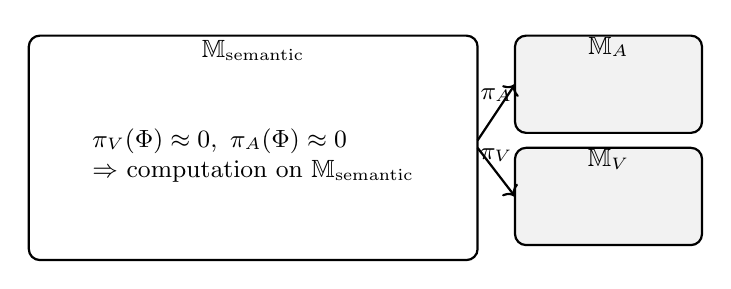
\begin{tikzpicture}[scale=0.95, every node/.style={font=\small}]
% Semantic box
\draw[rounded corners, thick] (0,0) rectangle (6,3);
\node at (3,2.8) {$\M_{\text{semantic}}$};
% Visual subspace
\draw[rounded corners, thick, fill=gray!10] (6.5,0.2) rectangle (9,1.5);
\node at (7.75,1.35) {$\M_V$};
% Auditory subspace
\draw[rounded corners, thick, fill=gray!10] (6.5,1.7) rectangle (9,3);
\node at (7.75,2.85) {$\M_A$};
% Arrows
\draw[->, thick] (6,1.5) -- (6.5,0.85) node[midway,above] {$\pi_V$};
\draw[->, thick] (6,1.6) -- (6.5,2.35) node[midway,above] {$\pi_A$};
% Aphantasia labels
\node[align=left] at (3,1.4) {$\pi_V(\Phi)\approx 0,\ \pi_A(\Phi)\approx 0$\\ $\Rightarrow$ computation on $\M_{\text{semantic}}$};
\end{tikzpicture}
\caption{Cognitive manifold with visual ($\M_V$) and auditory ($\M_A$) projections. Aphantasia/anendophasia suppress $\pi_V,\pi_A$ without impairing base dynamics.}
\label{fig:proj}
\end{figure}

% --------------------- 5. MIMETIC PROXIES (COX) ---------------------
\section{Mimetic Proxies (Cox) and Embodied Resonance}\label{sec:cox-mimetic}

\subsection{Cox’s Mimetic Hypothesis}
Cox’s hypothesis: understanding and imagination recruit covert motor simulation; perception is grounded in \emph{enacted} gesture. In music, MMI posits that we covertly sing, bow, or finger along with heard patterns; similar enactments support language and action understanding.

\subsection{RSVP Formalization}
Let $\bm{\mathcal v}_{\text{emb}}$ be the embodied component of $\bm{\mathcal v}$. Define a coupling functional
\begin{equation}
\Lambda[\Phi,\bm{\mathcal v}_{\text{emb}}](x) = \int_\M G(x,x')\,\bm{\mathcal v}_{\text{emb}}(x')\,dV_{x'},
\end{equation}
where $G$ is a Green’s function for a haptic/ideomotor operator. The effective scalar potential becomes
\begin{equation}
\Phi_{\text{eff}} = \Phi + \lambda\, \diverg \Lambda[\Phi,\bm{\mathcal v}_{\text{emb}}].
\end{equation}
Cox’s MMI predicts that even without imagery or inner speech, $\bm{\mathcal v}_{\text{emb}}$ channels semantic computation via covert action templates.

\subsection{Embodied Stigmergy}
When actions externalize (gesture, sketch, manipulate), $\bm{\mathcal v}_{\text{emb}}$ writes to the environment (Sec.~\ref{sec:stigmergy}), creating persistent traces that stabilize $S$ and guide future computation (stigmergic loops).

% --------------------- 6. AMPLITWISTOR + CPG ---------------------
\section{Midbrain Modulation and Amplitwistor Dynamics}\label{sec:amplitwistor}

\subsection{Central Pattern Generators (CPGs)}
CPGs in brainstem and basal ganglia provide rhythmic templates that entrain cortical networks via thalamocortical loops. We model their influence by a time-varying coupling tensor $\mathsf{C}_{ij}(t)$.

\subsection{Amplitwistor Modes}
Define synchronized submanifolds $\Sigma_k\subset \M$ and amplitwistor modes
\begin{equation}\label{eq:Ak}
\mathcal{A}_k(t) = \int_{\Sigma_k} \Phi(x,t)\, e^{i\omega_k t + p_k\cdot x}\, d^3x.
\end{equation}
Their evolution:
\begin{equation}\label{eq:Ak-evol}
\dot{\mathcal{A}}_k = -\sum_{i,j}\mathsf{C}_{ij}(t)\,\partial_j \Phi_i + i\omega_k \mathcal{A}_k - \gamma_k \mathcal{A}_k + \sum_{n=0}^{N}\beta_n \Gamma_k^{(n)},
\end{equation}
where $\Gamma_k^{(n)}$ are TARTAN/CLIO drives.

\begin{theorem}[Linear Stability]\label{thm:stab}
Linearizing \eqref{eq:Ak-evol} near $\mathcal{A}_k=0$ yields eigenvalues $\lambda_k$ with $\Re(\lambda_k)<0$ if $\gamma_k$ exceeds the largest real part induced by $\mathsf{C}(t)$ and drive terms. Thus low-gain sensory modes decay (aphantasia/anendophasia) while semantic modes may persist.
\end{theorem}

\subsection{Phase Synchronization (Kuramoto Order)}
Let $\theta_k=\arg(\mathcal{A}_k)$. The order parameter $r e^{i\Theta} = \frac{1}{N}\sum_k e^{i\theta_k}$ indexes coherence. Aphantasia predicts low $r$ in visual clusters under imagery demands but normal/compensated $r$ in task-relevant frontal-parietal clusters.

% --------------------- 7. TARTAN ---------------------
\section{TARTAN: Recursive Tiling and Entropy Geometry}\label{sec:tartan}
TARTAN partitions $\M$ into tiles $\tau_a^{(n)}$ at scale $n$, with local entropy tensor
\begin{equation}
\E_{ij}^{(n,a)} = \int_{\tau_a^{(n)}} (\partial_i S)(\partial_j S)\, w_\Phi\, d^3x,\qquad
w_\Phi = \frac{\Phi}{\int_{\tau_a^{(n)}} \Phi\, d^3x}.
\end{equation}
Renormalization across scales:
\begin{equation}
\E^{(n+1)} = \mathcal{R}[\E^{(n)}] + \Xi^{(n)},
\end{equation}
where $\Xi^{(n)}$ encodes annotated noise (embodied/contextual perturbations).

\paragraph{Convergence.} Convergent principal directions across scales predict stable mimetic projection (vivid imagery). Divergence corresponds to imageless regimes: semantic computation remains, but cross-scale alignment needed for vivid rendering fails to lock.

\begin{figure}[H]
\centering
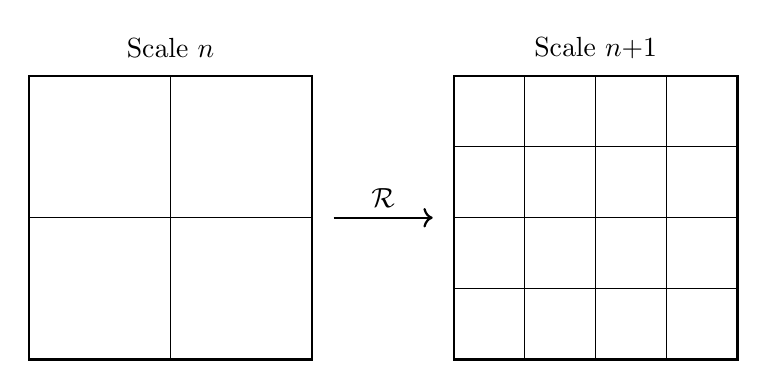
\begin{tikzpicture}[scale=0.9]
% Level n tiles
\draw[thick] (0,0) rectangle (4,4);
\draw (2,0)--(2,4);
\draw (0,2)--(4,2);
\node at (2,4.4) {Scale $n$};
% Level n+1 tiles
\draw[thick] (6,0) rectangle (10,4);
\foreach \x in {6,7,8,9,10} \draw (\x,0)--(\x,4);
\foreach \y in {0,1,2,3,4} \draw (6,\y)--(10,\y);
\node at (8,4.4) {Scale $n{+}1$};
% Arrows
\draw[->, thick] (4.3,2) -- (5.7,2) node[midway,above] {$\mathcal{R}$};
\end{tikzpicture}
\caption{TARTAN tiles coarsen/refine the manifold. Alignment of $\E^{(n)}$ principal directions signals emergent imagery; misalignment preserves imageless (semantic) dynamics.}
\label{fig:tartan}
\end{figure}

% --------------------- 8. CLIO ---------------------
\section{CLIO: Cognitive Loop via In-Situ Optimization}\label{sec:clio}
CLIO adapts parameters $\theta=(\{\omega_k\},\{\gamma_k\},\ldots)$ to task context via a free-energy-like objective:
\begin{equation}\label{eq:F}
\mathcal{F}(\theta) = \sum_n \alpha_n\, \mathrm{Tr}(\mathsf{G}\,\E^{(n)}(\theta)) + \lambda_1 \sum_k \norm{\nabla_\theta \omega_k}^2 + \lambda_2 \sum_k (\gamma_k - \gamma_k^\star)^2,
\end{equation}
with gradient update (momentum form)
\begin{equation}
\theta_{t+1} = \theta_t - \kappa_{\text{CLIO}} \nabla_\theta \mathcal{F}(\theta_t) + \mu(\theta_t-\theta_{t-1}).
\end{equation}
High loop gain can push sensory modes above threshold (vivid projections); subcritical gain sustains the \emph{silent base}.

\begin{figure}[H]
\centering
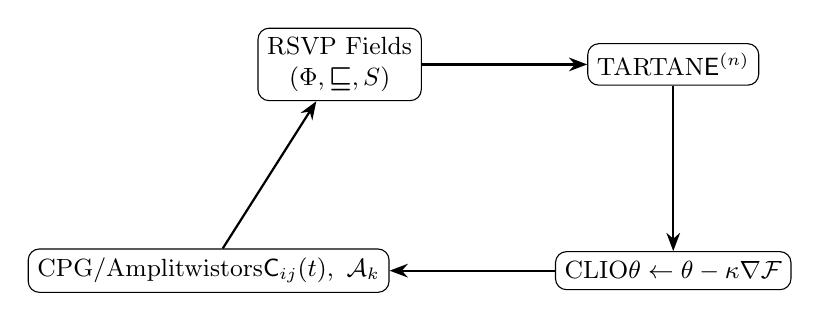
\begin{tikzpicture}[node distance=2.1cm, >=Stealth, every node/.style={font=\small}]
\node[draw, rounded corners, align=center] (fields) {RSVP Fields\\ $(\Phi,\bm{\mathcal v},S)$};
\node[draw, rounded corners, right=of fields] (tartan) {TARTAN\\ $\E^{(n)}$};
\node[draw, rounded corners, below=of tartan] (clio) {CLIO\\ $\theta\gets\theta-\kappa\nabla \mathcal F$};
\node[draw, rounded corners, left=of clio] (cpg) {CPG/Amplitwistors\\ $\mathsf C_{ij}(t),\ \mathcal{A}_k$};
\draw[->, thick] (fields) -- (tartan);
\draw[->, thick] (tartan) -- (clio);
\draw[->, thick] (clio) -- (cpg);
\draw[->, thick] (cpg) -- (fields);
\end{tikzpicture}
\caption{Closed loop: RSVP $\to$ TARTAN $\to$ CLIO $\to$ CPG/amplitwistors $\to$ RSVP.}
\label{fig:clio-loop}
\end{figure}

% --------------------- 9. STIGMERGY ---------------------
\section{Environmental Stigmergy as Interactive Memory}\label{sec:stigmergy}

\subsection{Coupled Internal--External Fields}
Let $\Phi_{\text{int}},\Phi_{\text{ext}}$ evolve by
\begin{align}
\partial_t \Phi_{\text{int}} &= D_{\text{int}}\Delta \Phi_{\text{int}} + \kappa_c(\Phi_{\text{ext}}-\Phi_{\text{int}}), \label{eq:phi-int}\\
\partial_t \Phi_{\text{ext}} &= D_{\text{ext}}\Delta \Phi_{\text{ext}} + \chi\, \bm{\mathcal v}_{\text{agent}}\cdot \grad \Phi_{\text{int}} - \delta \Phi_{\text{ext}}, \label{eq:phi-ext}
\end{align}
with Robin flux across the interface $\Sigma$:
\begin{equation}
D_{\text{int}}\grad \Phi_{\text{int}}\cdot n = D_{\text{ext}} \grad \Phi_{\text{ext}}\cdot n = \sigma(\Phi_{\text{ext}}-\Phi_{\text{int}}).
\end{equation}
These equations implement read/write between agent and artifacts (paper, screen, workspace).

\subsection{Information-Theoretic Capacity}
Define stigmergic capacity
\begin{equation}
\mathcal{C} := \sup_{\text{protocols}} I(\Phi_{\text{int}};\Phi_{\text{ext}}),
\end{equation}
subject to rate/distortion constraints determined by $D_{\text{ext}},\delta,\sigma,\chi$. Aphantasic strategies predict higher reliance on $\Phi_{\text{ext}}$ to maintain $\mathcal{C}$.

% --------------------- 10. QUANT + EXPERIMENTS ---------------------
\section{Quantitative Modeling and Experimental Predictions}\label{sec:quant-exp}

\subsection{Discretization and Parameters}
Use finite elements: P2 for scalars $(\Phi,S)$, Raviart--Thomas for $\bm{\mathcal v}$. Semi-implicit Crank--Nicolson in time, periodic or no-flux BCs.

\begin{table}[H]
\centering
\caption{Typical RSVP parameters (dimensionless units)}
\begin{tabular}{@{}ll@{}}
\toprule
Parameter & Value \\
\midrule
$\gamma$ & 0.5 \\
$\alpha$ & 0.10 \\
$\beta$  & 0.05 \\
$\kappa$ & 0.01 \\
$\omega_k$ & $4$--$100$ Hz \\
$\kappa_c$ & $0.2$ \\
$D_{\text{ext}}$ & $0.05$ \\
$\delta$ & $0.02$ \\
\bottomrule
\end{tabular}
\end{table}

\subsection{Predictions}\label{subsec:pred}
\begin{enumerate}
\item \textbf{Occipital gain:} During mental rotation, aphantasic V1/V2 shows lower beta power ($13$--$30$ Hz) than controls; fronto-parietal coupling is preserved (or enhanced).
\item \textbf{Stigmergic equalization:} Diagramming reduces group differences in reaction time/accuracy (effect size $d<0.1$).
\item \textbf{CLIO gain vs. VVIQ:} Estimated $\kappa_{\text{CLIO}}$ negatively correlates with VVIQ vividness.
\item \textbf{MMI without imagery:} EMG shows covert or minimal motor activation during semantic tasks in aphantasia; imagery tasks shift load to embodied channels.
\end{enumerate}

\subsection{Protocols}
\emph{Neuroimaging:} fMRI ROI in V1, PPC; DCM for connectivity.\\
\emph{EEG/MEG:} Time--frequency analyses; phase--amplitude coupling; $r$ (Kuramoto) in visual vs. frontal clusters.\\
\emph{Behavioral:} Shepard--Metzler rotation with/without external aids; reading under articulatory suppression for anendophasia.\\
\emph{Perturbation:} TMS to M1 or V1; tDCS to modulate gain; measure effects on $\mathcal{A}_k$ proxies.

% --------------------- 11. COMPARISONS + PHIL ---------------------
\section{Comparative Architectures and Philosophical Implications}\label{sec:comp-phil}
RSVP subsumes:
\begin{itemize}
\item \textbf{Predictive processing:} $S$ as a free-energy proxy; descent in \eqref{eq:s}.
\item \textbf{Global workspace:} high $\Phi$ supports broadcast; amplitwistors align phases.
\item \textbf{Attention schema:} $\mathsf{C}_{ij}(t)$ implements gain and meta-control.
\end{itemize}
Philosophically, representation is field-theoretic; phenomenology corresponds to boundary conditions and bifurcations (projection thresholds). Wordless/imageless thought is not a deficit but a regime in parameter space.


% --------------------- 12. LIMITATIONS + FUTURE --------------------- \section{Limitations and Future Work}\label{sec:limits-future} The present formulation of the RSVP cognitive field remains an approximation. Several conceptual and methodological limitations delimit its scope: \paragraph{Coarse Field Approximation.} Equations~\eqref{eq:phi}--\eqref{eq:s} coarse-grain neural and phenomenological activity into continuous scalar--vector fields. Spiking statistics, synaptic delays, and neurotransmitter dynamics are compressed into a diffusive term. While this abstraction captures macroscopic entropy flow, it cannot yet reproduce the discrete precision timing of cortical microcircuits or the high-frequency oscillatory cascades reported in laminar electrophysiology. Bridging this scale gap requires hybrid models that couple RSVP PDEs to stochastic point-process ensembles or mean-field neural mass formalisms. \paragraph{Parameter Identification and Empirical Mapping.} Coefficients $(\alpha,\beta,\gamma,\kappa,\ldots)$ are phenomenological; empirical identification demands multimodal datasets—EEG, fMRI, kinematics, and behavioral metrics—fit by variational inference or Hamiltonian Monte Carlo. Present fits are qualitative, based on dimensional analysis and approximate stability criteria. Future work should define canonical units and normalize entropy fluxes against metabolic expenditure or information-theoretic capacity, enabling reproducible parameter comparisons across laboratories. \paragraph{Analytical Gaps.} Global existence and uniqueness of the full stochastic coupled system remain open problems. The presence of multiplicative noise and nonlinear cross-coupling terms prevents standard energy-estimate proofs. Extending current local well-posedness results (Theorem \ref{thm:lwp}) will require compactness techniques, martingale formulations, or pathwise mild-solution constructions analogous to those in stochastic Navier–Stokes or reaction–diffusion theory. Such results would ground RSVP mathematically alongside classical physical field theories. \paragraph{Computational Constraints.} Simulations to date operate on coarse lattices ($32^3$–$64^3$ cells). Scaling to neurobiological resolution will demand GPU-parallel solvers with adaptive meshes, implicit time-stepping, and field compression through tensor networks or neural operators. A major priority is implementing the TARTAN–CLIO loop in real time to permit online parameter adaptation and closed-loop experiments. \paragraph{Neural and Phenomenological Correlates.} The mapping from field variables to measurable brain signals remains heuristic. For example, $\Phi$ is associated with semantic potential or metabolic availability, but its neural substrate could correspond to synaptic gain, dendritic voltage fields, or mesoscale BOLD fluctuations. Establishing empirical correlates will require simultaneous acquisition of behavioral, electrophysiological, and metabolic data under systematically varied imagery and speech conditions. \paragraph{Human-in-the-Loop Stigmergic Interfaces.} The proposed coupling between internal and external fields (\S\ref{sec:stigmergy}) has yet to be realized in interactive hardware. Developing writable, sensor-rich environments that register $\Phi_{\text{ext}}$ in real time—digital canvases, haptic controllers, or adaptive architectural surfaces—would permit direct measurement of stigmergic flux and enable cognitive feedback experiments. Such systems could serve both as research tools and as assistive interfaces for individuals with aphantasia or anendophasia. \paragraph{Ethical and Societal Dimensions.} Empirical deployment raises privacy and autonomy concerns: measuring entropic flux or stigmergic interaction may inadvertently quantify aspects of internal thought. Protocols must therefore embed ethical constraints at the level of instrumentation, not merely at data governance. The RSVP framework’s emphasis on distributed, entropy-respecting computation suggests designs that decentralize storage and analysis, aligning with the theory’s own thermodynamic ethics. \paragraph{Future Directions.} Immediate priorities include: \begin{enumerate}[label=(\alph*)] \item Deriving multiscale reductions linking RSVP fields to established neural field equations (Wilson–Cowan, Jansen–Rit). \item Constructing GPU-accelerated TARTAN/CLIO simulators with live visual feedback. \item Calibrating parameters via joint behavioral–neuroimaging experiments on imagery vividness and inner speech. \item Developing stigmergic laboratory environments for externalized cognition studies. \item Extending mathematical analysis to stochastic global existence and bifurcation classification. \item Exploring ethical architectures for entropy-aware, human-machine co-adaptation. \end{enumerate} In summary, RSVP presently offers a consistent phenomenological field theory uniting aphantasia, anendophasia, and embodied cognition under a single dynamical grammar. Its limitations are those of scale, proof, and instrumentation; its promise lies in closing those gaps through rigorous mathematics, empirical grounding, and technological embodiment. 

% --------------------- Appendices ---------------------
\appendix
\section{Derivation of the RSVP Field Equations}
\label{app:derivation}

The governing equations \eqref{eq:phi}--\eqref{eq:s} follow from a variational
principle on the Lagrangian density
\[
\mathcal{L}
= \frac{1}{2}g^{\mu\nu}(\nabla_\mu \Phi)(\nabla_\nu \Phi)
-\frac{\gamma}{2} g_{\mu\nu}\mathcal{v}^\mu \mathcal{v}^\nu
+\alpha\, S\log S
-\frac{\beta}{2} (\nabla\times\boldsymbol{\mathcal{v}})^2
-\kappa |\nabla S|^2 .
\]
The Euler--Lagrange operator on a field \(X\) is
\(
\mathcal{E}_X(\mathcal{L}) =
\frac{\partial \mathcal{L}}{\partial X}
- \nabla_\mu \frac{\partial \mathcal{L}}{\partial (\nabla_\mu X)}.
\)
Applying this to \(\Phi\), \(\boldsymbol{\mathcal{v}}\), and \(S\) yields
\begin{align*}
\partial_t \Phi &= -\nabla\!\cdot(\Phi\boldsymbol{\mathcal{v}})+\xi(t),\\
\partial_t \boldsymbol{\mathcal{v}} &=
(\nabla \Phi)\times\boldsymbol{\mathcal{v}}
-\gamma\boldsymbol{\mathcal{v}}
+\nabla\!\cdot(\mathsf{D}\nabla\boldsymbol{\mathcal{v}})+\boldsymbol{\eta}(t),\\
\partial_t S &=-\boldsymbol{\mathcal{v}}\!\cdot\!\nabla S
+\alpha\|\nabla\Phi\|^2
+\beta\|\nabla\times\boldsymbol{\mathcal{v}}\|^2
+\kappa\Delta S.
\end{align*}
By Noether’s theorem, time-translation invariance conserves total energy
\(E=\int(\tfrac12\Phi^2+\tfrac12|\boldsymbol{\mathcal{v}}|^2+\alpha S)\,dV\),
and gauge symmetry in \(\Phi\) implies an entropy current
\(J_S=S\boldsymbol{\mathcal{v}}-\kappa\nabla S\)
with continuity equation \(\partial_t S+\nabla\!\cdot J_S=0\).

\section{TARTAN: Recursive Tiling and Renormalization}
\label{app:tartan}

TARTAN (\emph{Trajectory-Aware Recursive Tiling with Annotated Noise})
constructs multiscale partitions of the manifold
\(\mathbb{M}\) into tiles \(\tau_a^{(n)}\).
Each tile carries local entropy tensor
\(\mathsf{E}_{ij}^{(n,a)}=\int_{\tau_a^{(n)}}(\nabla_i S)(\nabla_j S)\,w_\Phi\,d^3x\)
with weight \(w_\Phi=\Phi/\!\int_{\tau_a^{(n)}}\Phi\).
Renormalization across scales obeys
\[
\mathsf{E}^{(n+1)} = \mathcal{R}[\mathsf{E}^{(n)}]+\Xi^{(n)},
\]
where \(\mathcal{R}\) preserves invariant directions and
\(\Xi^{(n)}\) represents annotated noise injected by embodied context.

\paragraph{Algorithm (pseudo-code)}
\begin{verbatim}
for n in range(N_scales):
    for tile τ_a^(n) in partition(ℳ):
        compute E_ij^(n,a)
    E^(n+1) = R[E^(n)] + Ξ^(n)
\end{verbatim}

Convergence of \(\mathsf{E}^{(n)}\) signals emergence of coherent imagery;
divergence corresponds to the imageless (aphantasic) regime.

\section{CLIO: Cognitive Loop via In-Situ Optimization}
\label{app:clio}

CLIO implements recursive free-energy minimization over parameters
\(\theta=(\omega_k,\gamma_k)\).
Define the objective functional
\[
\mathcal{F}(\theta)
= \sum_n \alpha_n \mathrm{Tr}(\mathsf{G}\mathsf{E}^{(n)}(\theta))
  +\lambda_1\sum_k\|\nabla_\theta\omega_k\|^2
  +\lambda_2\sum_k(\gamma_k-\gamma_k^\star)^2.
\]
Gradient descent with momentum gives
\[
\theta_{t+1}
=\theta_t-\kappa_{\mathrm{CLIO}}\nabla_\theta\mathcal{F}
+\mu(\theta_t-\theta_{t-1}).
\]
In biological terms, this corresponds to local synaptic plasticity rules
driven by prediction error and stabilized by neuromodulators.

\section{Stigmergic Field Equations and Boundary Conditions}
\label{app:stig-eq}

Let the skin or tool interface define a surface \(\Sigma\subset\partial\mathbb{M}\).
Internal and external scalar potentials satisfy
\[
\begin{aligned}
\partial_t\Phi_{\text{int}}
 &=D_{\text{int}}\Delta\Phi_{\text{int}}
 +\kappa_c(\Phi_{\text{ext}}-\Phi_{\text{int}}),\\[2mm]
\partial_t\Phi_{\text{ext}}
 &=D_{\text{ext}}\Delta\Phi_{\text{ext}}
 +\chi(\boldsymbol{\mathcal{v}}_{\text{agent}}\!\cdot\!\nabla\Phi_{\text{int}})
 -\delta\Phi_{\text{ext}}.
\end{aligned}
\]
Continuity of flux across \(\Sigma\) gives the Robin-type condition
\[
D_{\text{int}}\nabla\Phi_{\text{int}}\!\cdot\!n
= D_{\text{ext}}\nabla\Phi_{\text{ext}}\!\cdot\!n
= \sigma(\Phi_{\text{ext}}-\Phi_{\text{int}}),
\]
where \(n\) is the outward normal and \(\sigma\) the coupling coefficient.
These equations govern write/read processes between cognition and environment.
Their discretization yields stable finite-element schemes for simulating
stigmergic cognition.

% --------------------- REFERENCES ---------------------
\begin{thebibliography}{99}\setlength\itemsep{0.2em}

\bibitem{Galton1880}
F. Galton, ``Statistics of Mental Imagery,'' \emph{Mind} \textbf{5} (1880), 301--318.

\bibitem{Zeman2015}
A. Zeman, M. Dewar, S. Della Sala, ``Lives without imagery: Congenital aphantasia,'' \emph{Cortex} \textbf{73} (2015), 378--380.

\bibitem{Faw2009}
T. Faw, ``MX: A Case of Lifelong Aphantasia,'' \emph{Consciousness and Cognition} \textbf{18} (2009), 331--334.

\bibitem{Fulford2018}
J. Fulford \emph{et al.}, ``The neural correlates of mental imagery in aphantasia,'' \emph{Cortex} (2018).

\bibitem{Keane2021}
B. Keane \emph{et al.}, ``Anendophasia: Investigating the loss of inner speech,'' \emph{Neuropsychologia} (2021).

\bibitem{Cox2001}
A. Cox, ``The Mimetic Hypothesis and Embodied Musical Meaning,'' \emph{Music Theory Online} \textbf{7}(1) (2001).

\bibitem{Cox2016}
A. Cox, \emph{Music and Embodied Cognition: Listening, Moving, Feeling, and Thinking}, Indiana University Press (2016).

\bibitem{Cox2021}
A. Cox, ``Mimetic Motor Imagery: Evidence and Implications,'' in \emph{Oxford Handbook of Music and the Body} (2021).

\bibitem{Clark1997}
A. Clark, \emph{Being There: Putting Brain, Body, and World Together Again}, MIT Press (1997).

\bibitem{Buzsaki2006}
G. Buzsáki, \emph{Rhythms of the Brain}, Oxford University Press (2006).

\bibitem{Muller2018}
L. Muller \emph{et al.}, ``Cortical traveling waves: mechanisms and computational roles,'' \emph{Nature Reviews Neuroscience} \textbf{19} (2018), 255--268.

\bibitem{EvansPDE}
L. C. Evans, \emph{Partial Differential Equations}, 2nd ed., AMS (2010).

\bibitem{Kuramoto}
Y. Kuramoto, \emph{Chemical Oscillations, Waves, and Turbulence}, Springer (1984).

\bibitem{Friston2010}
K. Friston, ``The free-energy principle: a unified brain theory?,'' \emph{Nature Reviews Neuroscience} \textbf{11} (2010), 127--138.

\bibitem{Bonabeau1999}
E. Bonabeau, M. Dorigo, G. Theraulaz, \emph{Swarm Intelligence: From Natural to Artificial Systems}, OUP (1999).

\bibitem{Wittgenstein1953}
L. Wittgenstein, \emph{Philosophical Investigations}, Blackwell (1953).

\end{thebibliography}


\end{spacing}
\end{document}